\documentclass{article}
% Language setting
% Replace `english' with e.g. `spanish' to change the document language
\usepackage[english]{babel}


% Set page size and margins
% Replace `letterpaper' with `a4paper' for UK/EU standard size
\usepackage[a4paper,top=2cm,bottom=2cm,left=3cm,right=3cm,marginparwidth=1.75cm]{geometry}

% Useful packages
\usepackage[utf8]{inputenc}
\usepackage{fontspec} 
\setmonofont{Fira Code}[Scale=0.9]

\usepackage{array}
\usepackage[most]{tcolorbox} % for inline code
\usepackage{amsmath}
\usepackage{graphicx}
\usepackage{subfigure}
\usepackage[colorlinks=true, allcolors=blue]{hyperref}
\usepackage{authblk}
\usepackage{amssymb}
\usepackage{listings}
\usepackage{color}
\usepackage{xcolor}
\usepackage{float}
\usepackage{biblatex} %Imports biblatex package
\addbibresource{references.bib} %Import the bibliography file
\usepackage{wrapfig}

\renewcommand{\floatpagefraction}{0.1}
\renewcommand{\textfraction}{0}

\definecolor{dkgreen}{rgb}{0,0.6,0}
\definecolor{gray}{rgb}{0.5,0.5,0.5}
\definecolor{mauve}{rgb}{0.58,0,0.82}
\definecolor{lightgray}{gray}{0.9}

\lstdefinestyle{pythonstyle}{
  language=Python,
  frame=tb,
  aboveskip=3mm,
  belowskip=3mm,
  showstringspaces=false,
  columns=flexible,
  basicstyle={\ttfamily\small},
  numbers=left,
  numberstyle=\tiny\color{gray},
  keywordstyle=\color{blue},
  commentstyle=\color{green!50!black},
  stringstyle=\color{red!70!black},
  breaklines=true,
  breakatwhitespace=true,
  tabsize=4,
  captionpos=b,
  morekeywords={self, cls, __init__, None},
}

\lstdefinestyle{pseudocode}{frame=tb,
  language=Python,
  aboveskip=3mm,
  belowskip=3mm,
  showstringspaces=false,
  columns=flexible,
  basicstyle={\small\ttfamily},
  numbers=left,
  numberstyle=\tiny\color{gray},
  keywordstyle=\color{blue},
  commentstyle=\color{dkgreen},
  stringstyle=\color{mauve},
  breaklines=true,
  breakatwhitespace=true,
  tabsize=3
}

\lstdefinestyle{input}{frame=none,
  aboveskip=3mm,
  belowskip=3mm,
  showstringspaces=false,
  columns=flexible,
  basicstyle={\small\ttfamily},
  numbers=none,
  numberstyle=\tiny\color{gray},
  keywordstyle=\color{blue},
  commentstyle=\color{dkgreen},
  stringstyle=\color{mauve},
  breaklines=true,
  breakatwhitespace=true,
  tabsize=3,
  captionpos=b,
}

% inline code display
\newtcbox{\inlinecode}{
  nobeforeafter, 
  colback=lightgray, 
  colframe=white, 
  boxrule=0pt, 
  arc=1mm, 
  left=0pt, right=0pt, top=0pt, bottom=0pt,
  on line,
  fontupper=\scriptsize\ttfamily
}


% make title
\title{
\includegraphics[scale=0.2]{Cam_logo_bw.png}\\
\vspace{0.5cm}
M1 Machine Learning Coursework
}
\author{xl628}
\affil{Department of Physics, University of Cambridge}

\begin{document}

\maketitle

\vspace{1cm}
\noindent
\textbf{Document Statistics:} \\
Words in text: 1736 \\
Words in headers: 82 \\
Words outside text (captions, etc.): 560 \\
Number of headers: 34 \\
Number of floats/tables/figures: 13 \\
Number of math inlines: 5 \\
Number of math displayed: 1


%----------------------------------------------------------------------------------
\section{Introduction}
The MNIST Addition task involves creating a synthetic dataset where pairs of digits from the MNIST dataset are combined to form an image, and their sum serves as the label. This report documents the methodology for generating this dataset, the implementation of a neural network pipeline optimized using Optuna, and the comparison of performance with Random Forest, Support Vector Machine (SVM), and Linear Classifiers. We also analyze the underlying data and model representations using t-SNE visualizations to demonstrate the effectiveness of our optimal model.

%----------------------------------------------------------------------------------
\section{Dataset Generation}

The primary implementation for dataset generation is located in \texttt{notebooks/data\_generation\_a} \texttt{nalysis.ipynb}.

\subsection{Implementation: \inlinecode{\small MNISTAdditionDataset} class}

The dataset is created using the \inlinecode{MNISTAdditionDataset} class, defined in \texttt{src/data\_handler.py}. Key methods and features include:

\paragraph{Normalization and Concatenation} The MNIST dataset is normalized from [0, 255] to [0, 1] upon loading. Two random digits are sampled with replacement and concatenated horizontally via the \inlinecode{\_combine\_images} method:

\begin{lstlisting}[style=pythonstyle, caption=Code snippet for \inlinecode{\_combine\_images}]
indices = np.random.choice(len(images), size=(num_samples, 2), replace=True)
combined_images = np.zeros((num_samples, 28, 56))
combined_labels = labels[indices].sum(axis=1)
digit_labels = labels[indices]

for i in range(num_samples):
combined_images[i, :, :28] = images[indices[i, 0]]
combined_images[i, :, 28:] = images[indices[i, 1]]
\end{lstlisting}


\paragraph{Random Seed}
To ensure reproducibility, a default seed (42) is set during initialization.

\paragraph{Dataset Split}

The generated dataset is divided into training, validation, and test sets. We first use \inlinecode{\_combine\_images} twice to generate the training and test datasets. Next, we further split the training dataset into training and validation datasets. During this process, we do not apply shuffling again, as randomness was already ensured during sampling.

\label{para:tfdataset}
\paragraph{TensorFlow Dataset Creation}
For efficient batching and shuffling during training, the \inlinecode{get\_tf\_dataset} method converts the dataset into a \inlinecode{tf.data.Dataset} object. Shuffling is typically enabled for training and validation datasets but disabled for test datasets.

\begin{figure}[!htbp]
    \centering
    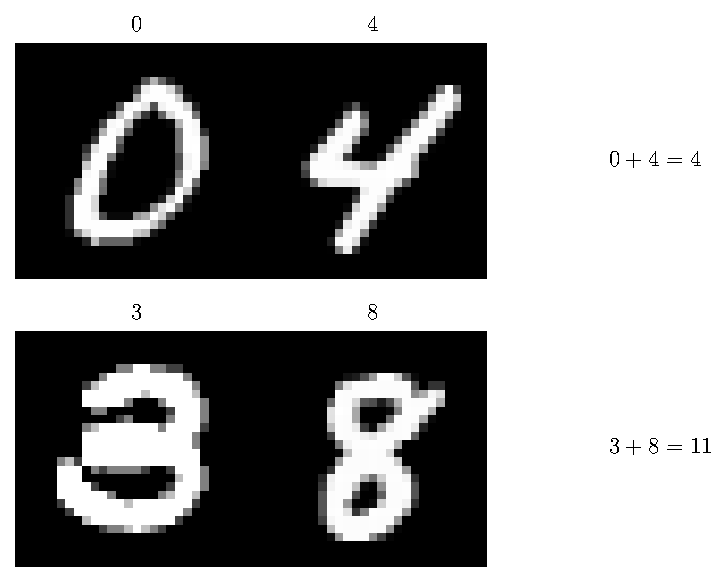
\includegraphics[width=0.6\linewidth]{./images/example_additions.pdf}
    \caption{The shape of the generated dataset is \inlinecode{(N, 28, 56)}, representing images of size 56 × 28 in computer dimensions. Here, N denotes the number of samples in the dataset. Two samples are randomly selected for visualization.}
\end{figure}


\subsection{Statistical Properties}

\begin{figure}[!htbp]
    \centering
    \subfigure[]{
        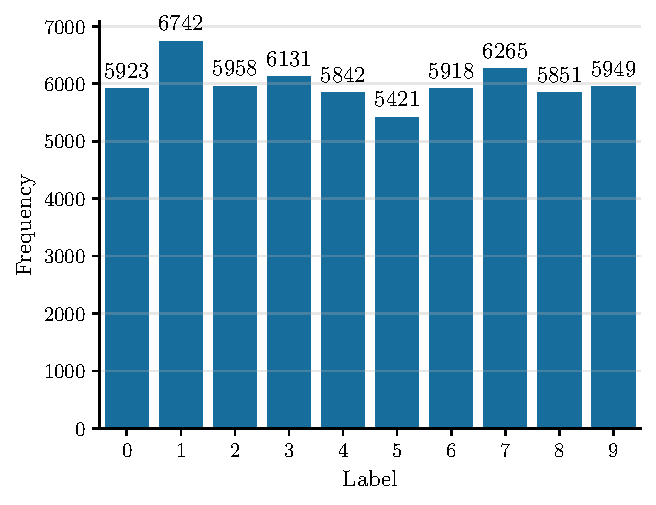
\includegraphics[width=0.47\textwidth]{./images/mnist_distribution.pdf}
        \label{fig:dist-1}
    }
    \hspace{0.0\textwidth}
    \subfigure[]{
        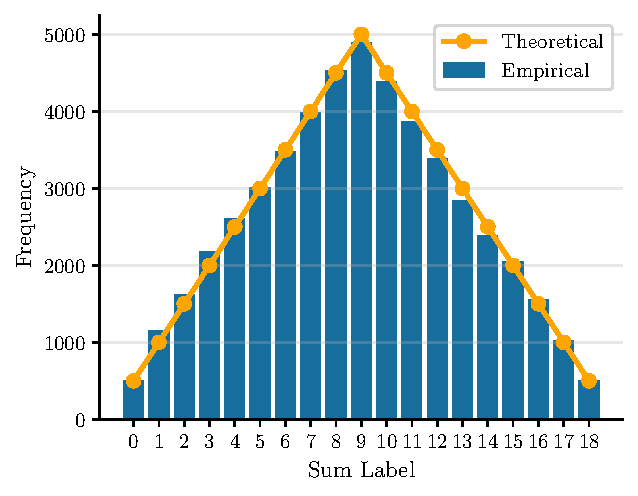
\includegraphics[width=0.47\textwidth]{./images/mnist_sum_distribution_combined.pdf}
        \label{fig:dist-2}
    }
    \caption{(a) The label distribution of the MNIST dataset.  
(b) The label distribution in the training set of the dataset generated by the default instance of the \inlinecode{MNISTAdditionDataset} class (i.e., using \inlinecode{dataset = MNISTAdditionDataset()} followed by \inlinecode{dataset.create\_datasets()}), containing a total of 50,000 data points. The orange line represents the theoretical distribution as defined in the equation \ref{eq:dist}, while the blue bars represent the empirical distribution.}
    \label{fig:two_dists}
\end{figure}

The generated dataset's quality is assessed through its statistical properties. Assuming that the original MNIST dataset is uniformly distributed, the generated dataset should theoretically follow a discrete triangular distribution.

\paragraph{Theoretical Distribution}
If \(X\) and \(Y\) are independent random variables uniformly distributed over the integers from 0 to 9, then their sum \( S = X + Y \) follows:

\begin{equation}
\label{eq:dist}
    P(S = s) =
    \begin{cases}
    \frac{s+1}{100} & \text{for } s=0,1,\ldots,9, \\
    \frac{19 - s}{100} & \text{for } s=10,11,\ldots,18.
    \end{cases}
\end{equation}

\paragraph{Empirical Analysis} Figures \ref{fig:dist-1} and \ref{fig:dist-2} compare the label distributions of the original and generated datasets. Results confirm alignment with theoretical expectations.


\section{Neural Network Pipeline}

The main notebook for this part is \texttt{notebooks/neural\_network\_optuna.ipynb}. And 
the main modules we will use in this section are \texttt{src/data\_handler.py} and \texttt{src/models.py}.


\subsection{Dataset Configurations}

We use the dataset generated by the default instance of the \inlinecode{MNISTAdditionDataset} class (e.g., \inlinecode{dataset = } \inlinecode{MNISTAdditionDataset(seed=42)} followed by \inlinecode{dataset.create\_datasets()}).

\begin{itemize}
\item \textbf{Training Dataset}: Input size \inlinecode{(50000, 28, 56)}; Output size \inlinecode{(50000,)}.
\item \textbf{Validation Dataset}: Input size \inlinecode{(10000, 28, 56)}; Output size \inlinecode{(10000,)}.
\item \textbf{Test Dataset}: Input size \inlinecode{(10000, 28, 56)}; Output size \inlinecode{(10000,)}.
\end{itemize}

\subsection{Baseline Model}
\label{sec:baseline}

The baseline fully connected neural network, detailed in \texttt{notebooks/neural\_network.ipynb}, achieves over 90\% test accuracy. This section outlines its configuration and chooses five hyper-parameters for further tuning.

\paragraph{TensorFlow Dataset} 
Key configurations include shuffled training and validation datasets (with fixed random seeds for reproducibility), a default batch size of 32, and \inlinecode{prefetch(tf.data.AUTOTUNE)}, which allows the pipeline to fetch and prepare the next batch of data asynchronously while the current batch is being processed, to optimize data pipeline efficiency.

\paragraph{Architecture} The neural network will be a normal fully connected network, with various hyper-parameters.
\begin{itemize}
    \item \textbf{Input and Output} - The input layer processes data of shape \inlinecode{(28, 56)}. After flattening, it outputs \inlinecode{(1568,)} (normally in row-major order). The final layer outputs \inlinecode{(19,)}.
    \item \textbf{Batch Normalization} - Applied after each activation function for stability and efficiency. Batch normalization can be strategically implemented between the linear transformation and the activation function; however, in this specific task, it is applied following each activation function.
    \item \textbf{Dropout} - Dropout layers follow batch normalization. The dropout rate will be a tunable hyper-parameter.
    \item \textbf{Dense Layers} - Fully connected layers will have three tunable parameters, including the number of layers, activation functions, and neurons.
\end{itemize}

\paragraph{Training}
\begin{itemize}
    \item \textbf{Optimizer} - The \inlinecode{Adam} optimizer is used, with a tunable learning rate.
    \item \textbf{Epochs} - Fixed at 50 to balance efficiency and overfitting.
    \item \textbf{Batch Size} - Set to 32.
    \item \textbf{Loss Function} - \inlinecode{sparse\_categorical\_crossentropy} is employed for simplicity. L2 regularization is added to dense layers to mitigate overfitting.
\end{itemize}

\subsection{Hyper-parameter Optimization with Optuna}

We optimize the number of dense layers, activation functions, neurons per layer, dropout rate, and learning rate.


\paragraph{Model Class}
The \inlinecode{DigitAdditionModel} class in \texttt{src/models.py} simplifies hyper-parameter testing and model management.

\paragraph{Optuna}
Optuna\cite{optuna} provides automated hyper-parameter optimization using efficient search algorithms. The key components include:

We implement a class \inlinecode{OptunaOptimizer} for this specific MNIST addition hyper-parameter tuning task for better organization.

\paragraph{Study}
Configured using \inlinecode{optuna.create\_study()}, which defines sampling and pruning algorithms:

Samplers basically continually narrow down the search space using the records of suggested parameter values and evaluated objective values, leading to an optimal search space which giving off parameters leading to better objective values. Pruners automatically stop unpromising trials at the early stages of the training (a.k.a., automated early-stopping).\cite{optuna_tutorial_efficient_algorithms}

We utilize the standard Tree-structured Parzen Estimator algorithm for sampling. Furthermore, a pruning algorithm is omitted because early-stopping, which is set by default, or other callback methods are integrated into each training session as defined in the \inlinecode{DigitAdditionModel} class.

\paragraph{Objective\cite{optuna_first_study}}
Evaluates each trial using \inlinecode{DigitAdditionModel.build()} and returns validation accuracy.

\paragraph{Optimization} 
We log the search process, store optimal parameters and model weights.

\paragraph{Running}
See \texttt{notebooks/neural\_network\_optuna.ipynb} for code, where we set the hyper-parameter search range and display results. 

Eventually, we present an overall report from a study of 20 trials:

\begin{lstlisting}[style=input, caption=Hyperparameter Optimization Results]
Final Results Summary:
Hyperparameter Optimization Results:
--------------------------------------------------

Best Trial:
  Value (Validation Accuracy): 0.9634
  Hyperparameters:
    n_layers: 4
    dropout_rate: 0.17753778267309397
    learning_rate: 0.00040593004933114283
    l2_reg: 1e-06
    activation: elu
    units_l0: 567
    units_l1: 215
    units_l2: 208
    units_l3: 823

Parameter Importance:
  units_l0: 0.4870
  n_layers: 0.3066
  learning_rate: 0.0712
  dropout_rate: 0.0632
  units_l1: 0.0558
  activation: 0.0162
  l2_reg: 0.0000
\end{lstlisting}
Parameter importance is evaluated using the fANOVA importance evaluator\cite{optuna_param_importances}, which fits a random forest regression model to predict objective values from parameter configurations of COMPLETE trials. The range of \texttt{l2\_reg} is non-tunable in our setting and fixed at (1e-6, 1e-6), resulting in an importance of 0.

The search log is in \texttt{notebooks/logs/optimization.log}, and the best parameters and model weights are saved in \texttt{notebooks/results/optimization\_results.json} and \texttt{notebooks/model} \texttt{s/best\_model\_weights.weights.h5}, respectively.

The inherent visualizations provided by Optuna reveal several interesting insights during the search process. Refer to Figure \ref{fig:three_figs} for details.

\begin{figure}[!htbp]
    \centering
    \subfigure[]{
    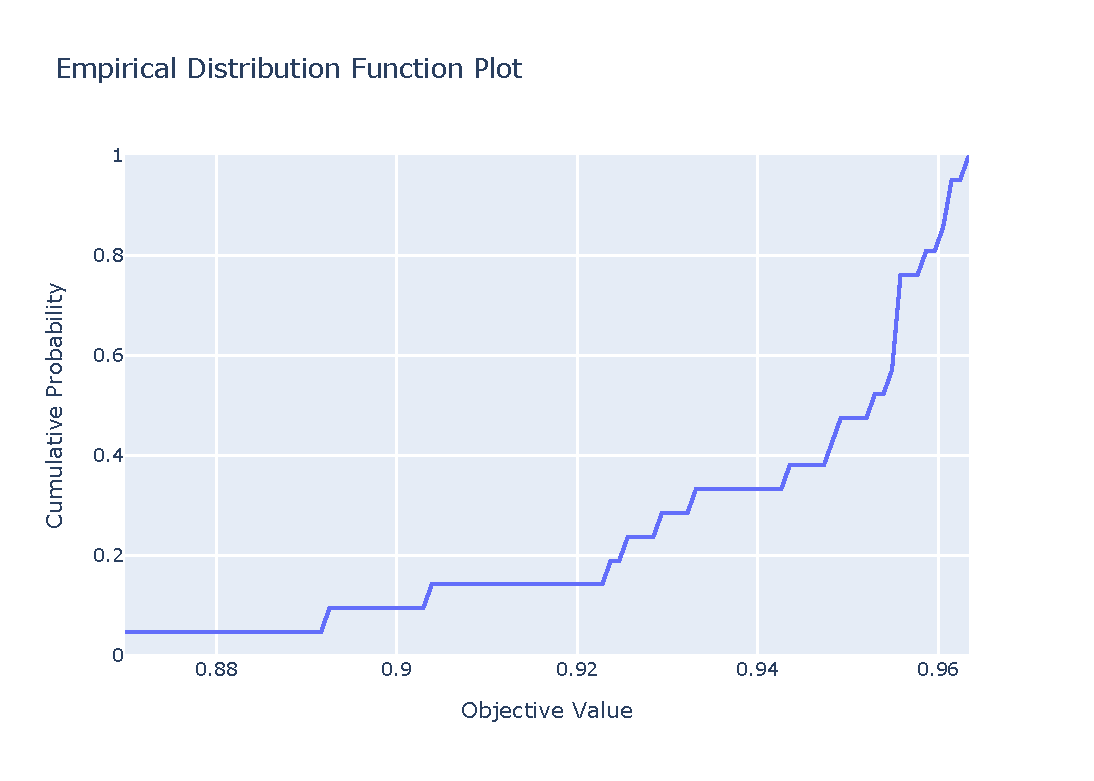
\includegraphics[width=0.475\textwidth]{./images/edf.pdf}
        \label{fig:edf}
    }
    \hspace{0.0\textwidth}
    \subfigure[]{
        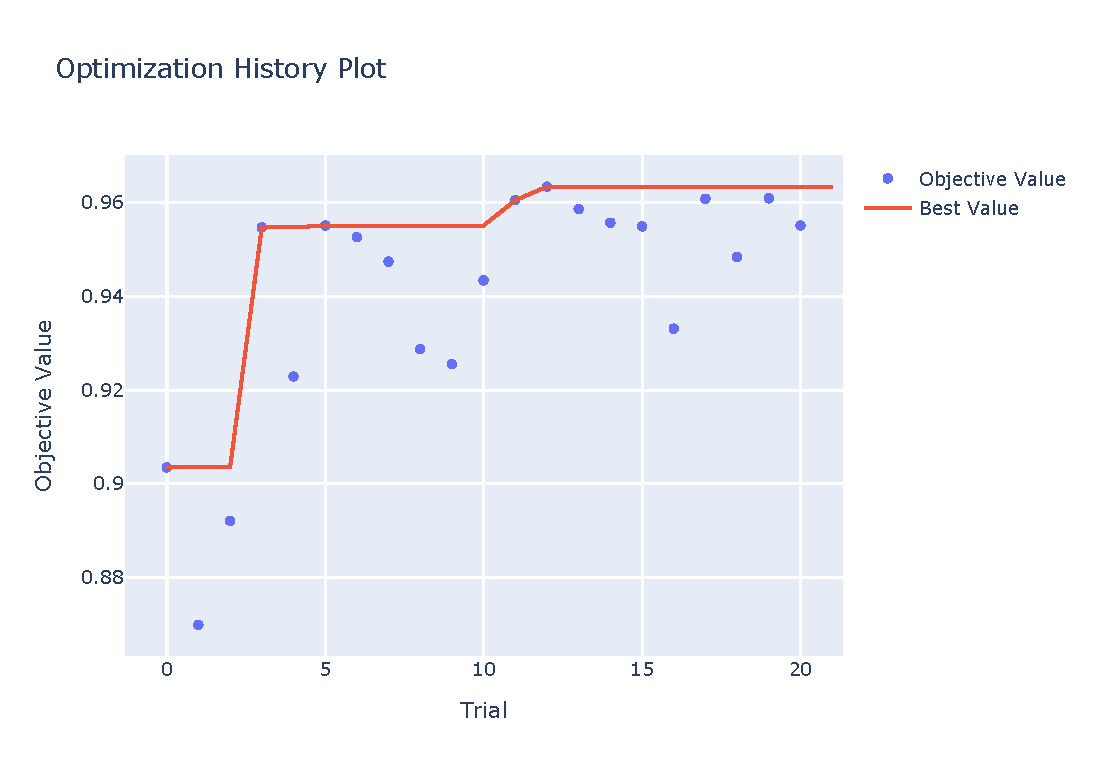
\includegraphics[width=0.475\textwidth]{./images/optimization_history.pdf}
        \label{fig:op-hist}
    }
    \hspace{0.0\textwidth}
    \subfigure[]{
        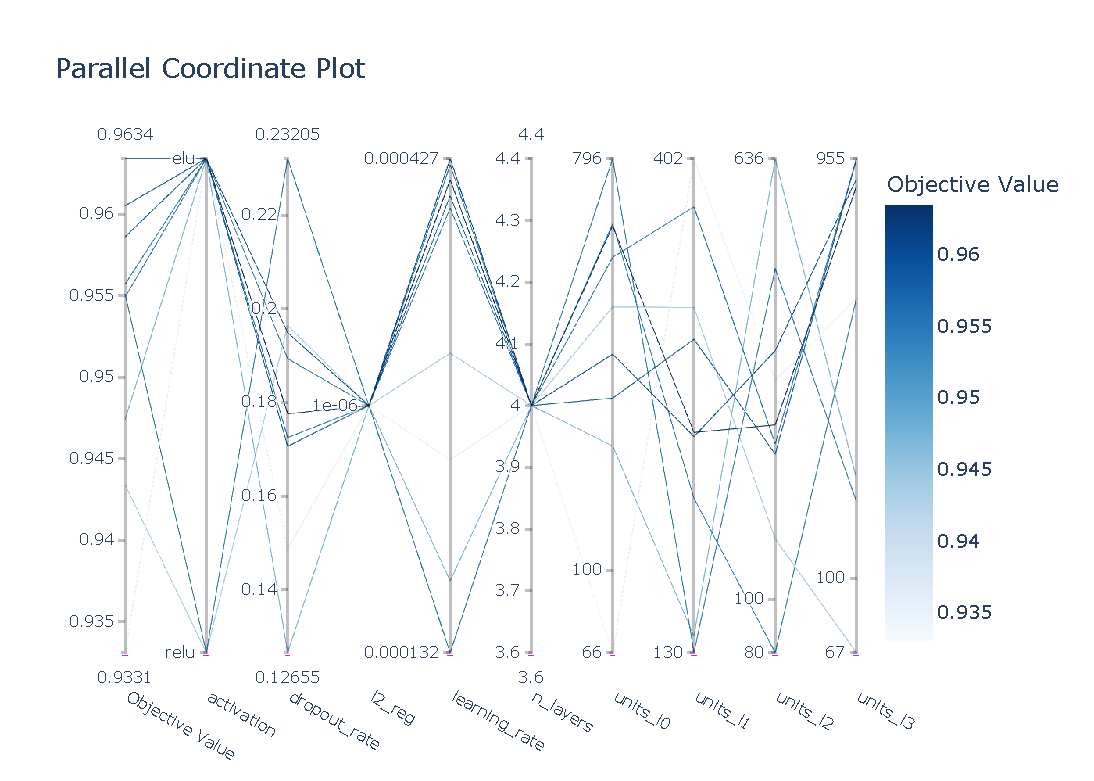
\includegraphics[width=0.7\textwidth]{./images/parallel_coordinate.pdf}
        \label{fig:op-pc}
    }
    \caption{The visualization module provided by Optuna was used to generate the plots for this search. (a) \textbf{The empirical cumulative distribution function (CDF) of the objective values} (highest validation accuracy corresponding to hyperparameters). Within the given search space, the accuracy of most models exceeds 90\%, and the probability density function seems to rise sharply after reaching 95\%, indicating that further improving accuracy beyond this point becomes increasingly challenging. (b) \textbf{Optimization history}. As the number of searches increases, the accuracy of the parameters found tends to improve, showcasing the advantage of the Optuna search algorithm. (c) \textbf{Path lines of parameter combinations}. Darker path lines represent parameter combinations with higher accuracy. Notable observations include: most searches utilized the \texttt{elu} activation function; for the \texttt{elu} activation function, a dropout rate of 0.17–0.2 tends to be more suitable. Learning rates generally performed better at higher or lower values within the illustrated range $[0.000132, 0.000427]$, with middling values performing less effectively. The value of \texttt{n\_layers} is generally better at 4, which is also the maximum set value, possibly indicating that more complex models might perform better. Additionally, configurations where the 1st and 4th hidden layers have more units, while the middle two hidden layers have relatively fewer units, tend to perform better.
}
    \label{fig:three_figs}
\end{figure}

\subsection{Optimal Model Evaluation}
\label{sec:optimalNN}

The architecute of the best model, as detailed in \texttt{notebooks/best\_neural\_network\_tsne.ipynb}, is summarized in Table \ref{table:nn_summary}. A visualization can be referred in Figure \ref{fig:nn}. For all other parameters, please refer to Section \ref{sec:baseline}.



\begin{table}[!htbp]
\centering
{\ttfamily
\begin{tabular}{|l|l|l|}
\hline
\textbf{Layer (type)}             & \textbf{Output Shape} & \textbf{Param \#} \\ \hline
input\_layer\_1 (InputLayer)      & (None, 28, 56)        & 0                 \\ \hline
flatten\_1 (Flatten)              & (None, 1568)          & 0                 \\ \hline
dense\_5 (Dense)                  & (None, 567)           & 889,623           \\ \hline
batch\_normalization\_4 (BatchNormalization) & (None, 567) & 2,268             \\ \hline
dropout\_4 (Dropout)              & (None, 567)           & 0                 \\ \hline
dense\_6 (Dense)                  & (None, 215)           & 122,120           \\ \hline
batch\_normalization\_5 (BatchNormalization) & (None, 215) & 860               \\ \hline
dropout\_5 (Dropout)              & (None, 215)           & 0                 \\ \hline
dense\_7 (Dense)                  & (None, 208)           & 44,928            \\ \hline
batch\_normalization\_6 (BatchNormalization) & (None, 208) & 832               \\ \hline
dropout\_6 (Dropout)              & (None, 208)           & 0                 \\ \hline
dense\_8 (Dense)                  & (None, 823)           & 172,007           \\ \hline
batch\_normalization\_7 (BatchNormalization) & (None, 823) & 3,292             \\ \hline
dropout\_7 (Dropout)              & (None, 823)           & 0                 \\ \hline
dense\_9 (Dense)                  & (None, 19)            & 15,656            \\ \hline
\end{tabular}
}
\caption{Neural Network Model Summary}
\label{table:nn_summary}
\end{table}

\begin{figure}[!htbp]
    \centering
    
\includegraphics[width=0.42\linewidth]{./images/best_nn_architecture.pdf}
    \caption{Architecture of the optimal fully connected neural network.}
\label{fig:nn}
\end{figure}


\begin{figure}[!htbp]

    \centering
    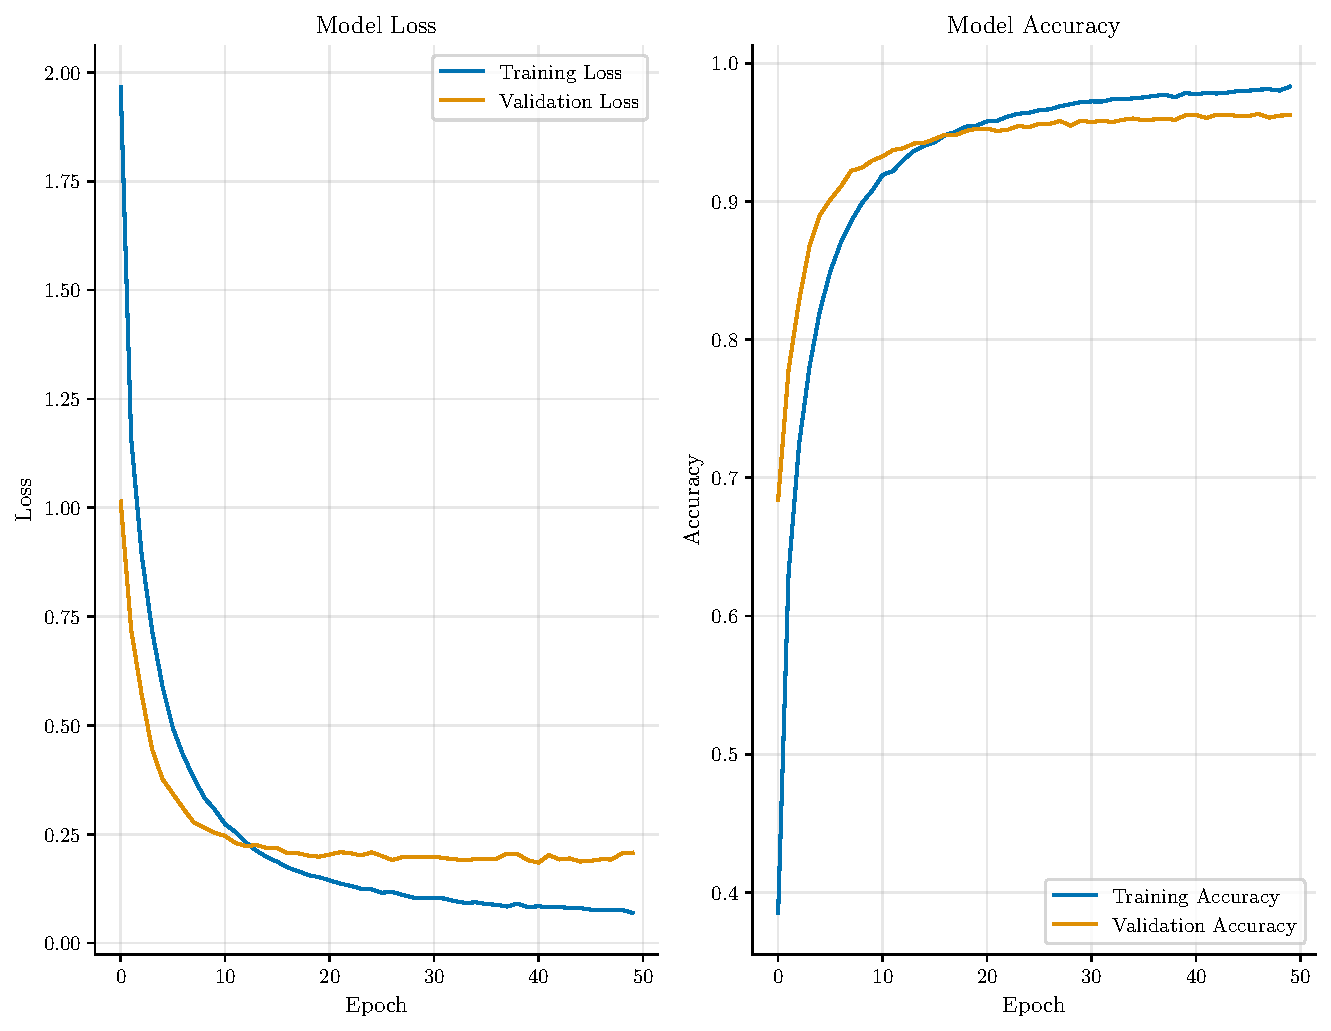
\includegraphics[width=0.8\linewidth]{./images/training_history.pdf}
    \caption{The loss and accuracy curves during the training process of the optimal model. It can be observed that after approximately the 20th epoch, the performance on the validation set stagnates, while the training set performance continues to improve, indicating a sign of overfitting.
}
\label{fig:curves}
\end{figure}

The optimal model achieved a test accuracy of 94.84\%. Training and validation curves (Figure \ref{fig:curves}) indicate potential overfitting after 20 epochs.

We visualize misclassified data in Figure \ref{fig:misclassified}. Some MNIST digits are indistinguishable even to humans, affecting accuracy and generalization.

\begin{figure}[!htbp]
    \centering
    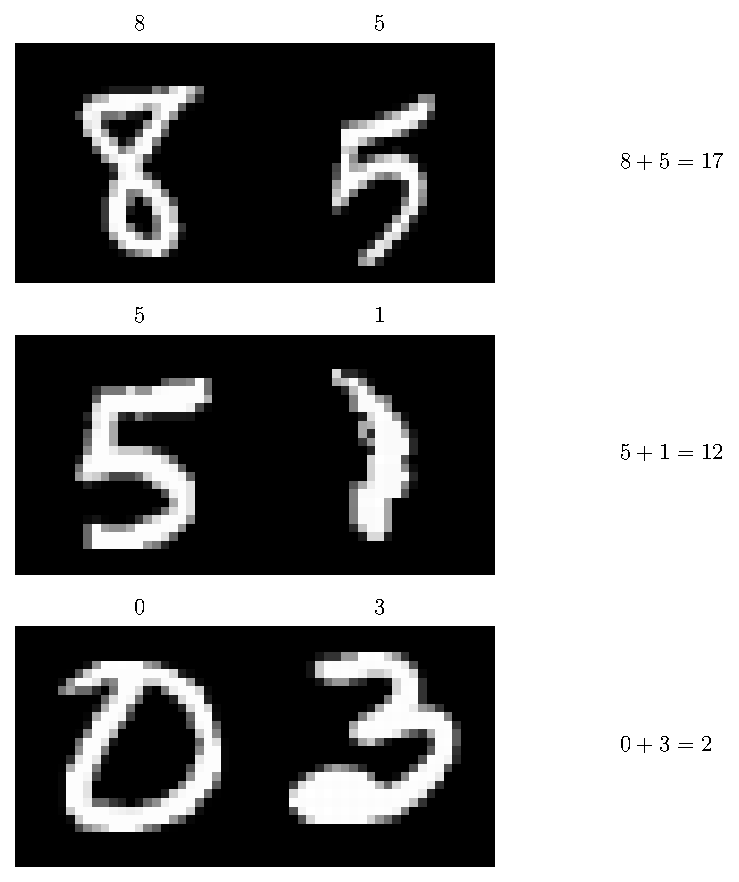
\includegraphics[width=0.6\linewidth]{./images/incorrect_predictions.pdf}
    \caption{Examples of some misclassified data on the test set.}
\label{fig:misclassified}
\end{figure}

\newpage

\section{Random Forest and Support Vector Machine}

This section provides an evaluation of the performance of Random Forest and Support Vector Machine (SVM) classifiers for the MNIST addition task.

The implementation is detailed in \texttt{notebooks/classifier\_comparison.ipynb}, where specific configurations are presented.

We use the flattened image as input. However, feature engineering, which is not discussed in this report, is also a significantly important and large topic. 

Moreover, given the non-uniform distribution of sample numbers across classes, certain techniques will be employed to mitigate this imbalance.

\paragraph{Random Forest}

Random Forest classifiers are robust ensemble learning models that aggregate decisions from multiple decision trees. 

An approach to address the issue of imbalance in Random Forest classifiers involves changing the split criterion during the tree construction process. Two fundamental criteria are \inlinecode{'gini'} and \inlinecode{'entropy'}.

\begin{itemize}
    \item \textbf{Gini Index} - The default criterion in \inlinecode{RandomForestClassifier} from \texttt{scikit-learn}. Gini Index measures the impurity of a dataset based on the probability of misclassifying a randomly chosen element. While computationally efficient, it may exhibit bias toward features with fewer categories.
    \item \textbf{Entropy} - Derived from information theory, entropy measures dataset impurity or disorder and uses information gain to optimize tree splits.
\end{itemize}

Moreover, using \inlinecode{class\_weight='balanced'} setting counteracts imbalance by automatically adjusting class weights inversely to their frequency, giving minority classes more attention in training \cite{scikit_learn_rf_classifier}.

Six Random Forest configurations were evaluated, with results summarized in Figure \ref{fig:rf}. Despite varied configurations, none surpassed the test accuracy of neural networks, with all models achieving less than 80\% accuracy.

\begin{figure}[!htbp]
    \centering
    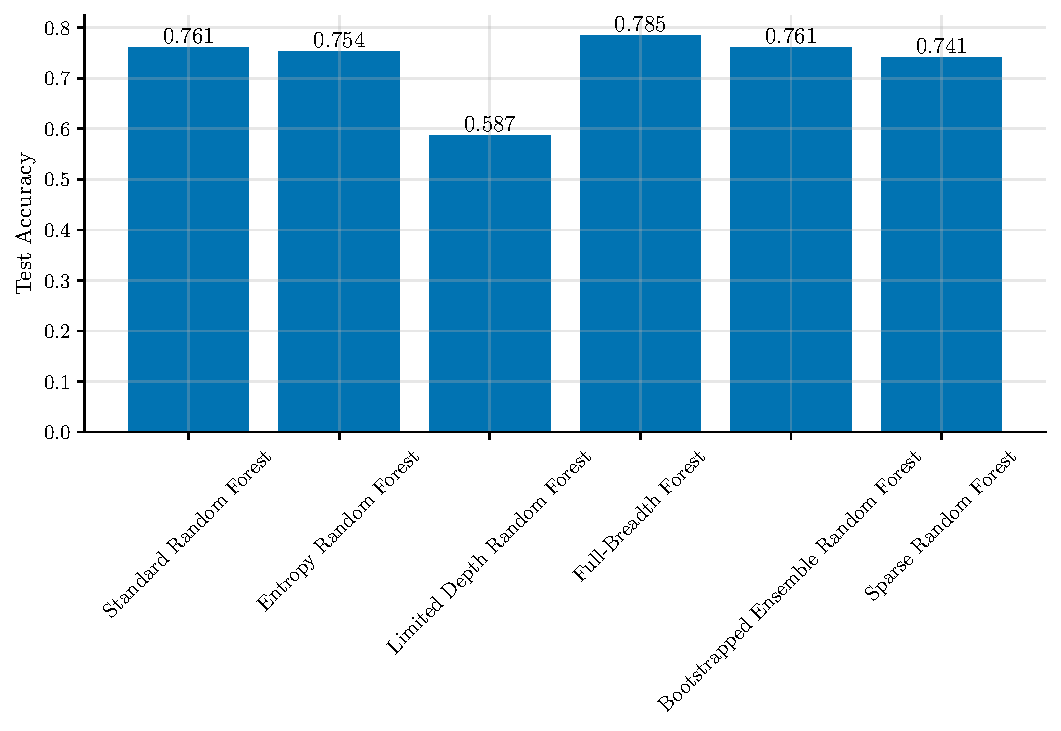
\includegraphics[width=0.8\linewidth]{./images/rf_comparison.pdf}
    \caption{Test accuracy for six Random Forest models. Limited Depth and Full-Breadth Forest configurations differ in tree depth, number of trees, and leaf node requirements. It has been shown that more complex Random Forest models perform better for this problem. The two models on the far right configure the \inlinecode{max\_samples} and \inlinecode{max\_features} used by each base learner, respectively.}
\label{fig:rf}
\end{figure}

\paragraph{Support Vector Machine (SVM)}
SVMs are computationally intensive, particularly on high-dimensional datasets like MNIST. Consequently, we trained SVM models on a reduced dataset comprising 40\% of the original training data.

Seven SVM configurations were tested, and their results are presented in Figure \ref{fig:svm}. Overall, SVMs performed worse than both Random Forest and neural networks. Linear Kernel SVM and low-penalty (C) RBF SVM especially exhibited lower performance.

\begin{figure}[!htbp]
    \centering
    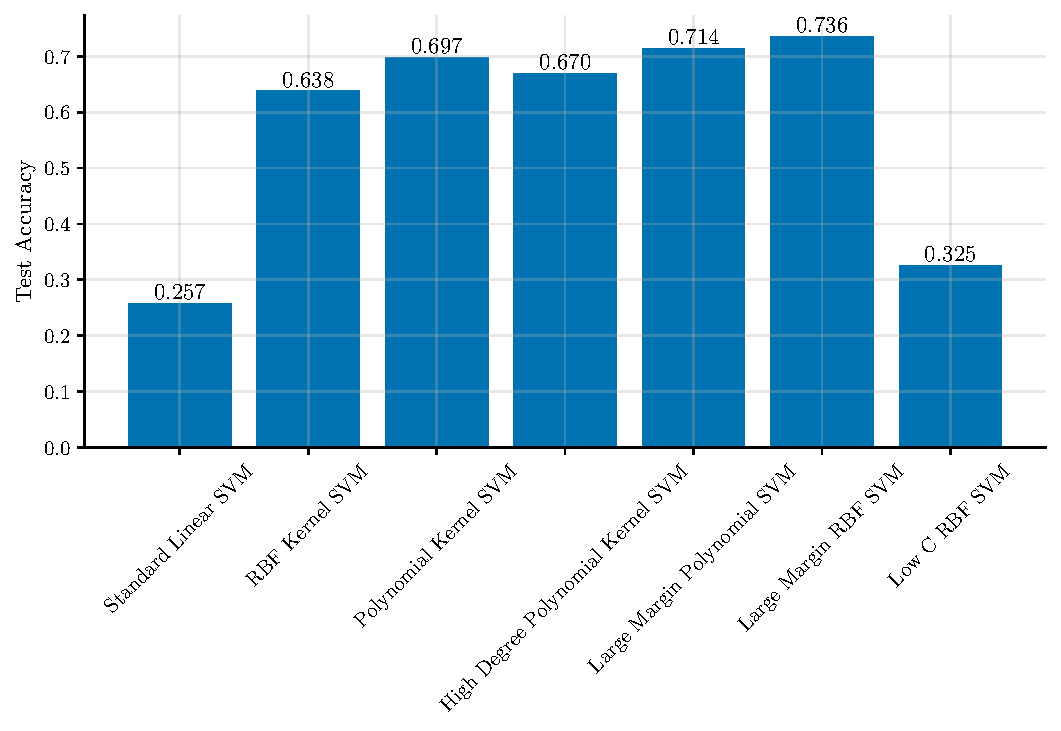
\includegraphics[width=0.8\linewidth]{./images/svm_comparison.pdf}
    \caption{Test accuracy for seven SVM configurations.}
\label{fig:svm}
\end{figure}

\section{Linear Classifiers}

In \texttt{notebooks/linear\_classifiers.ipynb}, we implement two types of classifiers on the $56\times 28$ dataset: the \textbf{Joint Classifier}, which predicts the sum directly, and the \textbf{Sequential Classifier}, which predicts each digit sequentially and then calculates their sum.

We evaluate these classifiers across various training set sizes (\texttt{[50, 100, 500, 1000, 10000, 50000]}) using a fixed test set size of \texttt{10000}. Figure \ref{fig:confidence} illustrates the average confidence for different training sizes and the confidence distribution for classifiers trained on the largest dataset (50000 samples). Confidence is defined as the highest softmax probability predicted for each test data point.

\begin{figure}[!htbp]
    \centering
    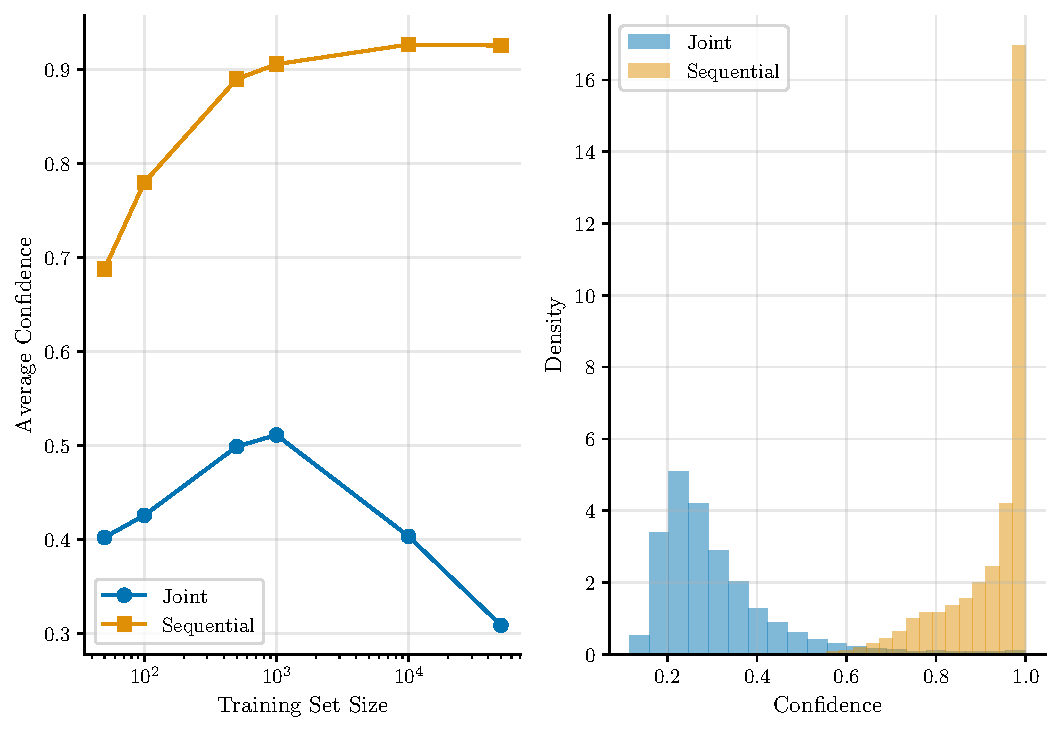
\includegraphics[width=0.8\linewidth]{./images/confidence_analysis.pdf}
    \caption{Left: Average confidence of the test set across different training set sizes. As the size increases, the confidence of the Joint Classifier decreases after a certain limit, whereas the Sequential Classifier improves, reaching 90\%. Right: Confidence distribution for the test set at a training size of 50,000.}
\label{fig:confidence}
\end{figure}

The test set performance is shown in Figure \ref{fig:linear}. The results indicate that the Sequential Classifier significantly outperforms the Joint Classifier in both accuracy and confidence,  making it a more effective design.

\begin{figure}[!htbp]
    \centering
    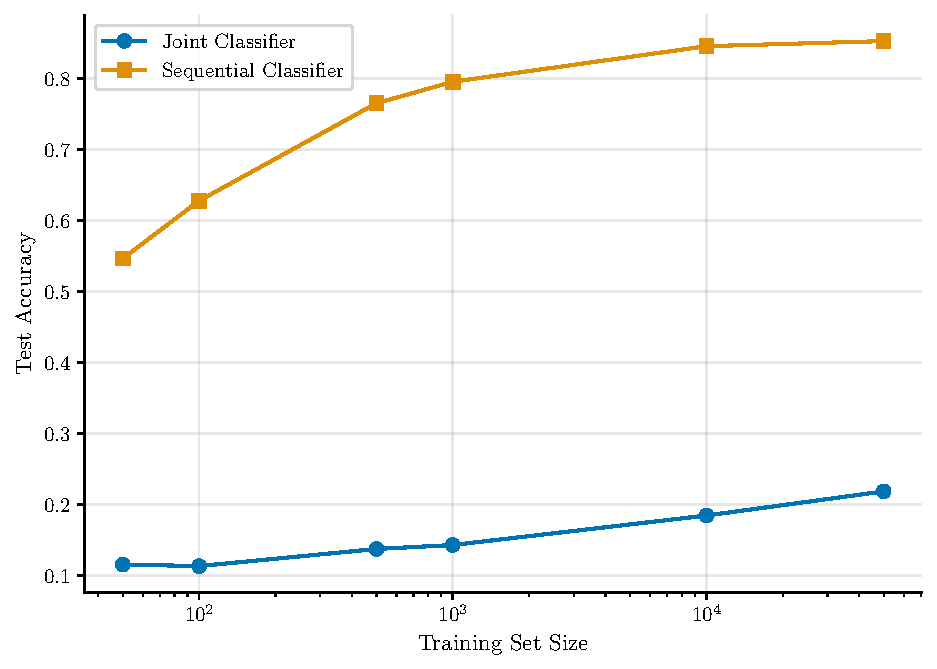
\includegraphics[width=0.8\linewidth]{./images/linear_classifier_comparison.pdf}
    \caption{Sequential Classifier accuracy steadily increases, surpassing 80\% as the training size grows. The Joint Classifier also improves but remains weak.}
\label{fig:linear}
\end{figure}

All in all, Sequential Classifier design has much higher confidence and accuarcy.

\section{t-Distributed Stochastic Neighbor Embedding (t-SNE) Distribution}

The t-SNE is a powerful dimensionality reduction technique. It projects high-dimensional data into lower-dimensional spaces, preserving meaningful structure.

\paragraph{Perplexity and Its Role}
Perplexity is a critical hyperparameter in t-SNE that balances global and local data structures. Higher perplexity emphasizes broader relationships, while lower values focus on local clustering.

In \texttt{notebooks/best\_neural\_network\_tsne.ipynb}, we visualize the first two t-SNE dimensions for the embedding layer of the optimal neural network (see Section \ref{sec:optimalNN}) and the raw input dataset. The chosen perplexity values result from multiple trials to optimize visualization.

The results, shown in Figures \ref{fig:embedding-tsne} and \ref{fig:input-tsne}, demonstrate that the neural network effectively transforms unstructured input data into meaningful feature representations within its embedding layer.

\begin{figure}[!htbp]
    \centering
    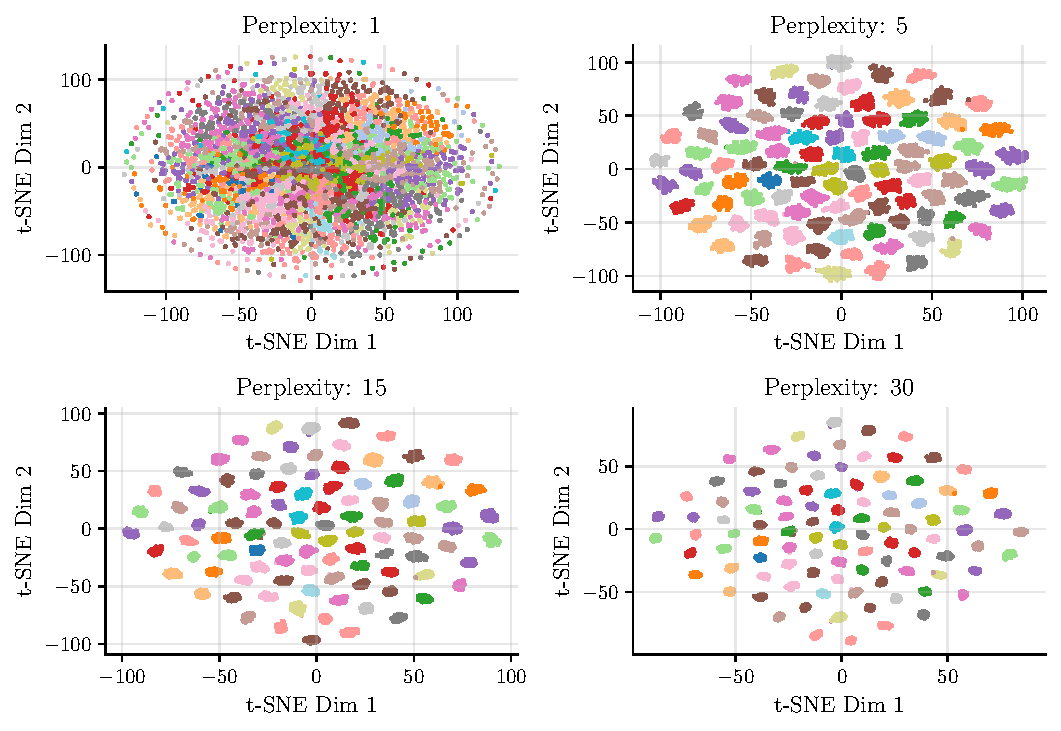
\includegraphics[width=0.9\linewidth]{./images/embeddings_tsne.pdf}
    \caption{t-SNE visualization of the embedding layer with different perplexity values. Clusters are evident at Perplexity=5. While 19 colors represent the 19 classes, the observed number of clusters exceeds 19, likely reflecting different additive combinations for the same sum.}
\label{fig:embedding-tsne}
\end{figure}

\begin{figure}[!htbp]
    \centering
    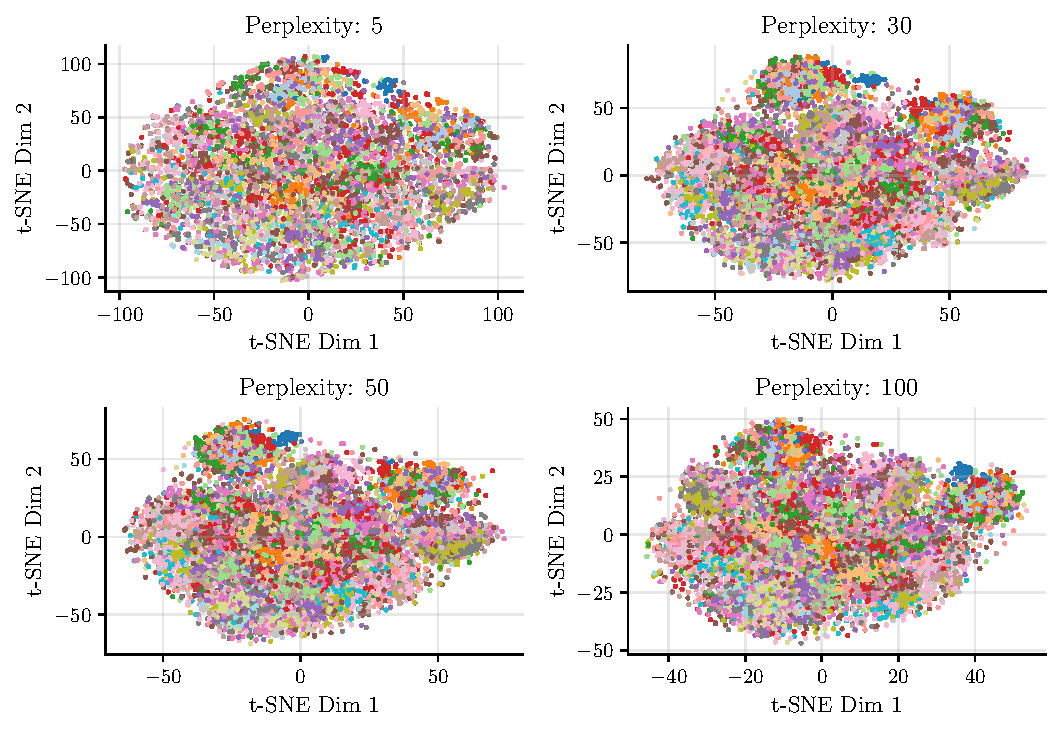
\includegraphics[width=0.9\linewidth]{./images/inputs_tsne.pdf}
    \caption{t-SNE visualization of the raw input dataset under various perplexity settings. No discernible structure emerges, regardless of perplexity.}
\label{fig:input-tsne}
\end{figure}

\section{Conclusion}
This study demonstrates that neural networks, particularly when optimized with advanced hyper-parameter tuning techniques like Optuna, outperform traditional machine learning models such as Random Forest and SVM for the MNIST Addition task. Sequential Classifier designs within linear classifiers also show promise, achieving competitive accuracy and confidence. Additionally, t-SNE visualizations highlight the capability of neural networks to transform unstructured input data into meaningful feature representations. These findings reinforce the importance of tailored model design and hyper-parameter optimization in achieving high performance.

\clearpage
\newpage
\appendix
\section{Use of AI Tools}
The following describes how AI tools were utilized in the preparation of this report:
\begin{itemize}
    \item ChatGPT 4o
        \begin{itemize}
            \item \textbf{Drafting} - Used for drafting certain sections of the report, including the Introduction, t-SNE section, Conclusion, and Appendix.
            \item \textbf{Proofreading} - Reviewed grammatical correctness, improved sentence structure, and suggested alternative wordings for clarity across the report.
            \item \textbf{LaTeX Assistance} - Helped resolve issues encountered during the LaTeX formatting process, such as debugging compilation errors, optimizing figure placement, and improving overall document layout.
        \end{itemize}
\end{itemize}

\section{Template Information}
This report was formatted using the LaTeX template from the given Example Coursework (by Michal Dorko). Some modifications were made.

\newpage
\printbibliography
\end{document}